%%%%%%%%%%%%%%%%%%%%%%%%%%%%%%%%%%%%%%%%%%%%%%%%%%%%%%%%%%%%%%%%%%%%%%
%     File: ExtendedAbstract_resul.tex                               %
%     Tex Master: ExtendedAbstract.tex                               %
%                                                                    %
%     Author: Andre Calado Marta                                     %
%     Last modified : 27 Dez 2011                                    %
%%%%%%%%%%%%%%%%%%%%%%%%%%%%%%%%%%%%%%%%%%%%%%%%%%%%%%%%%%%%%%%%%%%%%%
% Results
% Results should be clear and concise.
% Discussion
% This should explore the significance of the results of the work, not
% repeat them. A combined Results and Discussion section is often
% appropriate. Avoid extensive citations and discussion of published
% literature.
%%%%%%%%%%%%%%%%%%%%%%%%%%%%%%%%%%%%%%%%%%%%%%%%%%%%%%%%%%%%%%%%%%%%%%

\section{Results}
\label{sec:resul}

Place text here...


%%%%%%%%%%%%%%%%%%%%%%%%%%%%%%%%%%%%%%%%%%%%%%%%%%%%%%%%%%%%%%%%%%%%%%
\subsection{Sub-section...}

More text...

Figure~\ref{fig:blade_flow_pressure} shows the contour of pressure on the hub and blade surface planes corresponding to the baseline blade geometry.

\begin{figure}[H]
  \centering
  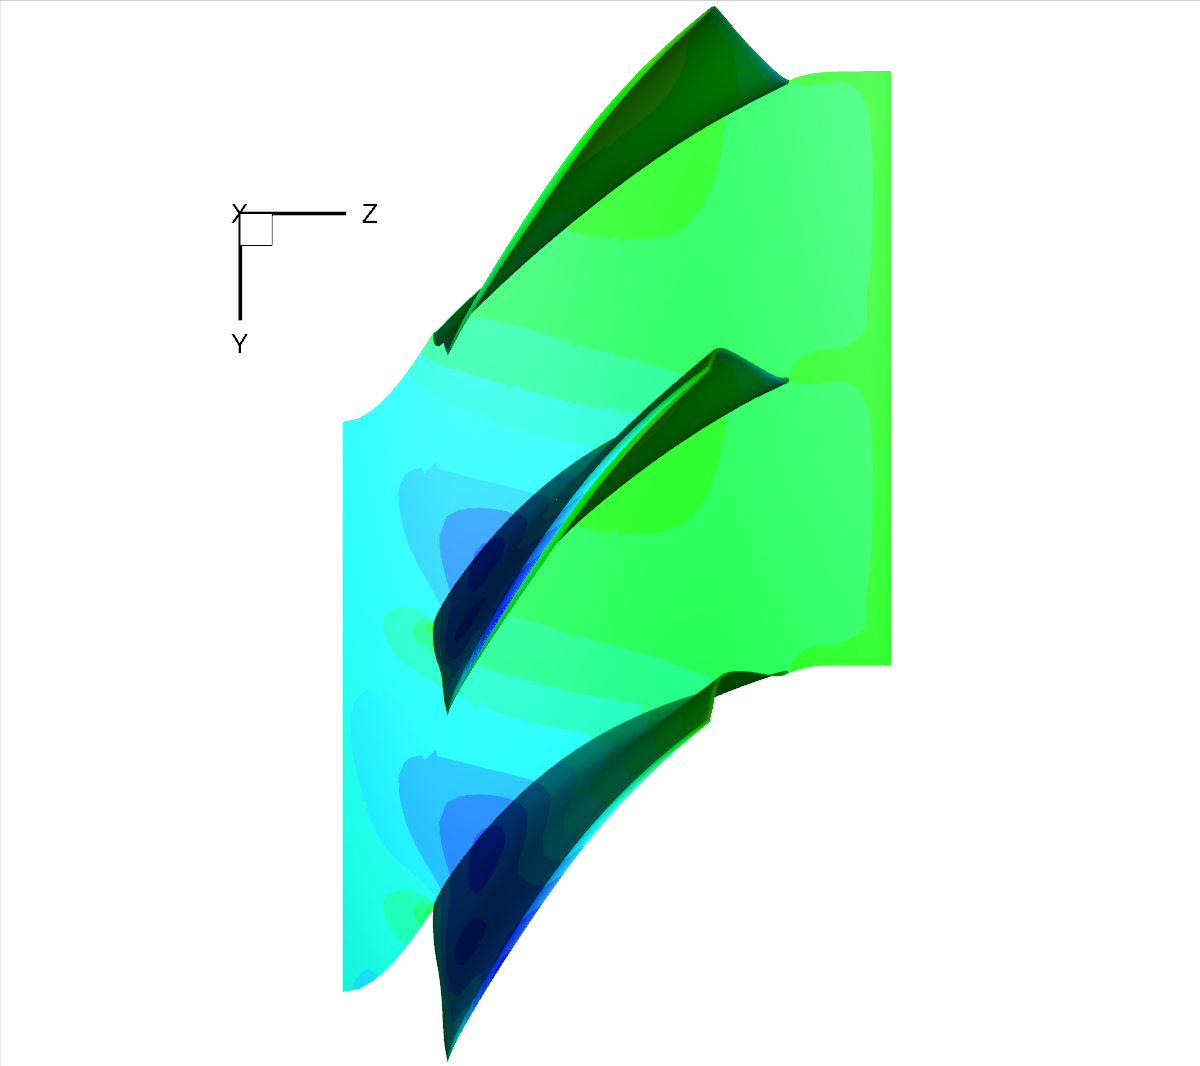
\includegraphics[width=5cm]{images/master_flow.png}
  \caption{Pressure distribution.}
  \label{fig:blade_flow_pressure}
\end{figure}

As seen in Fig.\ref{fig:blade_flow_pressure}...


%%%%%%%%%%%%%%%%%%%%%%%%%%%%%%%%%%%%%%%%%%%%%%%%%%%%%%%%%%%%%%%%%%%%%%
\subsection{Sub-section...}

More text...

Table~\ref{table:simple} summarizes...

\begin{table}[!h]
  \begin{center}
    \begin{tabular}{lccc}
      Model           & $C_L$ & $C_D$ & $C_{M y}$ \\
      \hline
      Euler           & 0.083 & 0.021 & -0.110    \\
      Navier--Stokes  & 0.078 & 0.023 & -0.101    \\
      \hline
    \end{tabular}
  \end{center}
  \caption[Table caption shown in TOC]{Table caption}
  \label{table:simple}
\end{table}

As seen in Tab.\ref{table:simple}...

